\documentclass[11pt, a4paper]{article}
\usepackage[utf8]{inputenc} 
\usepackage{fullpage}
\usepackage{graphicx}
\usepackage[hidelinks]{hyperref,xcolor}
\usepackage[left=0.5in, right=0.5in, top=0.5in, bottom=0.5in]{geometry}
\usepackage{tocbibind} % This package automatically adds bibliography to TOC
\usepackage{float}
\renewcommand\UrlFont{\color{blue}\rmfamily}

% Bibliography management
%  see https://www.overleaf.com/learn/latex/Biblatex_citation_styles
%  and https://www.overleaf.com/learn/latex/Bibliography_management_in_LaTeX
% to use overleaf with reference manager
%  see: https://no.overleaf.com/blog/639-tip-of-the-week-overleaf-and-reference-managers
% \usepackage[backend=biber]{biblatex}
% \addbibresource{library.bib} %Imports bibliography file
 
% Title of your project
\title{Drug potency prediction of SARS-Cov2-Mpro based on Graph Convolutional Network}

% Name of deliverable
\newcommand{\deliverableName}{MASTER’S Thesis FINAL PROJECT}

% Group names(s)
\author{Youssef Ezz Eldeen Ezzat}

% Group number
\newcommand{\groupNumber}{x}

% Any comments for us
\newcommand{\comments}{Comments for teachers of the course}

 % Web address for the project (if any)
\newcommand{\homepage}{\url{https://www.ntnu.edu/studies/courses/IT3010}}

% Date for title page, default is today
\date{\today}


\makeatletter{}

\begin{document}

% Title page based on https://www.latextemplates.com/template/academic-title-page
\begin{titlepage}

  	\newcommand{\HRule}{\rule{\linewidth}{0.3mm}} % Defines a new command for horizontal lines, change thickness here
	\center % Centre everything on the page
	%------------------------------------------------
	%	Headings
	%------------------------------------------------
	
	%------------------------------------------------
	%	Author(s)
	%------------------------------------------------

	% If you don't want a supervisor, uncomment the two lines below and comment the code above
 	%	{\large\textit{Author}}\\
	{\large\sc\@author}\\[1.5cm] % Your name

	\textsc{\LARGE MASTER’S DEGREE IN SECURITY ENGINEERING AND ARTIFICAL INTELLIGENCE (MESIIA)}\\[1.5cm]
	
	\textsc{\Large \deliverableName}\\[0.5cm]
	
	\textsc{\large Directed by Prof. Francesc Serratosa}\\[0.5cm]
	
	%------------------------------------------------
	%	Title
	%------------------------------------------------
	
	\HRule\\[0.4cm]
	
	{\huge\bfseries \@title}\\[0.4cm]
	
	\HRule\\[1.5cm]
	
	

 %   \footnotesize{Comments: \comments}
%   \vfill\vfill
%    \homepage
%    \vfill
    
    %------------------------------------------------
    % Change log for the plan (can be deleted before delivery)
    % When you update the plan please record what you changed and what the reason for the change. This will be useful for your supervisor.
    %------------------------------------------------
    % \input{./changelog.tex}
	
	%------------------------------------------------
	%	Logo
	%------------------------------------------------
	\vfill
	
\includegraphics[width=0.3\textwidth]{./urvlogo.png}\\[2.0cm]
	
	 
		
	%------------------------------------------------
	%	City
	%------------------------------------------------
	
	
	{\large Tarragona} % City

	
		
	%------------------------------------------------
	%	Date
	%------------------------------------------------
	
	{\large\@date} % Date, change the \today to a set date if you want to be precise
    \vfill
	
	
\end{titlepage}


\tableofcontents

\section{Introduction}


    A virus encodes one or more proteases which are enzymes that spur the formation of new protein products, thus play crucial roles in virus replication ,
    and are important targets for the design and development of potent antiviral agents or drugs.
    Binding affinity is the strength of the binding interaction between a single biomolecule (e.g., a virus protein) to its ligand or binding partner (e.g., a drug).
    it is a key to appreciating the intermolecular interactions driving biological processes and measured as part of the drug discovery process to help design drugs that bind their targets selectively and specifically.

    The development of new drugs is costly, time consuming and often accompanied with safety issues.
    Drug repurposing can avoid the expensive and lengthy process of drug development by finding new uses for already approved drugs. In order to repurpose drugs effectively, it is useful to know which proteins are targeted by
    which drugs which is the definition of Drug-Target-Affinity(DTA)\cite{1}

    there is a strong motivation to build computational models that can estimate the interaction strength of new drug–target pairs based on previous drug–target
    experiments.

    the DTA prediction problem as a regression task where the input is a drug–target pair and the output is a continuous measurement of binding affinity
    for that pair.

\section{Abstract}
    A graph, in general, is a data structure depicting a collection of entities represented as nodes, and
    their pairwise relationships represented as edges. There is a growing interest in having graph-based
    techniques applied to machine learning, for instance, in biotechnology, they are used to represent
    drugs and proteins in order to predict their binding affinity. The aim of this master thesis is to apply
    graph regression techniques based on graph convolutional networks (GCN) to predict the binding
    affinity of drugs and the SARS-Cov2 Mpro.
    \\Thus, the specific aim of this master thesis is to define and code in python a GCN to predict the
    binding affinity of a database generated in the URV composed of several pairs of the main protease
    of SARS-Cov2 and a drug.
    \\The master will include the theoretical explanations of
    \begin{itemize}
        \item Binding affinity prediction
        \item Graph Convolutional Networks    
    \end{itemize}
    And also the practical use of the following Python code \url{https://github.com/YoussefEzz/GraphDTA_forked} \cite{3} to perform the prediction.
    
\section{Drug Representation}
    \subsection{SMILES notation}
    Simplified Molecular Input Line Entry System (SMILES) was invented to represent molecules to be readable by computers.
    enabling several efficient applications, including
    fast retrieval and substructure searching. From the SMILES code,
    drug descriptors like the number of heavy atoms or valence electrons
    can be inferred and readily used as features for affinity prediction.
    One could also view the SMILES code as a string
    \begin{itemize}
        \item Methane: "C"
        \item Ethanol: "CCO"
        \item Benzene: "c1ccccc1" 
        \item Glucose: "OC[C@@H]1OC@HC@@HC@H[C@H]1O"     
    \end{itemize}
    for example the benzene molecule with the SMILES notation "c1ccccc1" has six carbon atoms in a circular and planar shape which can be inferred from the SMILES notation and 
    it's worth mentioning that this is a famous example of an aromatic molecule where aromaticity is an important feature of stability.
    \begin{figure}[H]
        \centering
        \begin{minipage}{0.2\textwidth}
        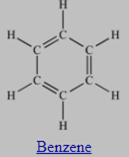
\includegraphics[width=\textwidth]{Benzene.png}
        \end{minipage}   
    \end{figure}

\section{Protein Representation}
    \subsection{Protein Sequence}
    A protein sequence is the order of amino acids in a protein. Amino acids are the building blocks of proteins, and there are about 20 different amino acids that can be found in proteins. The sequence of amino acids in a protein determines its three-dimensional structure and its function.
    so The sequence is a string of ASCII characters which represent amino
    acids. 
    \\Each amino acid type is encoded with an integer based on its
    associated alphabetical symbol [e.g. Alanine (A) is 1, Cystine (C) is
    3, Aspartic Acid (D) is 4 and so on], allowing the protein to be represented as an integer sequence.
    imagine a protein as a word. Each letter in the word represents an amino acid. The order of the letters in the word determines the meaning of the word. Similarly, the order of amino acids in a protein determines its function.
    \\ an example of a protein sequence, representing the first 7 amino acids of the protein insulin:
    \textbf{GIVEQCC...}
    This sequence represents the following amino acids:
    \begin{itemize}
        \item \textbf{G}: Glycine
        \item \textbf{I}: Isoleucine
        \item \textbf{V}: Valine 
        \item \textbf{E}: Glutamic acid
        \item \textbf{Q}: Glutamine
        \item \textbf{C}: Cysteine
        \item \textbf{C}: Cysteine    
    \end{itemize}

\section{Binding affinity measurements}
    \subsection{The kinase dissociation constant \textbf{kd}}
        It measures the equilibrium between the ligand(drug)-protein complex and the dissociated components. \\
        It corresponds to the affinity which the ligand has for the binding site. \\
        under usual conditions the dissociation constant gives the ligand concentration at which half of the protein molecules have ligand bound.\\
        Ligands with higher, more favorable free energy of association bind “tighter” and therefore have greater preference for the bound state. Because \textbf{kd} is defined as a dissociation constant, higher affinity ligands have lower \textbf{kd} values.\\ 
        As an equilibrium constant, we can express it as the ratio of product concentrations over reactants:
        \begin{figure}[H]
            \centering
            \begin{minipage}{0.45\textwidth}
            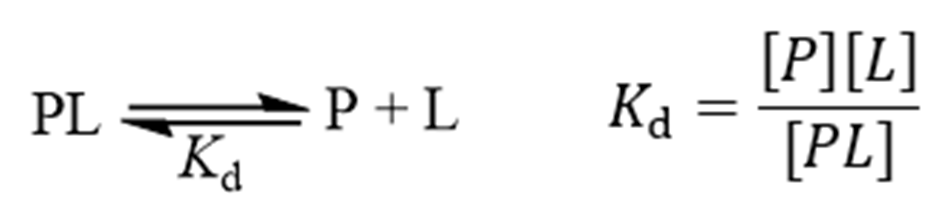
\includegraphics[width=\textwidth]{affinity measurements/kd.png}
            \end{minipage}   
        \end{figure}
        where
        \begin{itemize}
            \item [P] is the free protein concentration
            \item [L] is the free ligand concentration
            \item [PL] is the protein-ligand complex         
        \end{itemize}

    \subsection{The kinase Inhibition Constant \textbf{ki}}
        represents the affinity of the drug molecule for its target receptor, specifically in the context of competitive inhibition.

        \begin{figure}[H]
            \centering
            \begin{minipage}{0.45\textwidth}
            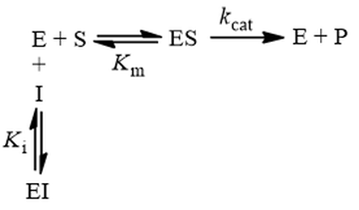
\includegraphics[width=\textwidth]{affinity measurements/ki.png}
            \end{minipage}   
        \end{figure}
        where
        \begin{itemize}
            \item [E] is the free enzyme concentration
            \item [I] is the inhibitor or drug
            \item [S] is the substrate or the molecules that an enzyme acts upon.
            \item [ES] is the enzyme-substrate complex concentration (ES)
            \item [P] is the product concentration which is the Protein in this case
            \item [km] is the Michaelis constant is a kinetic parameter, not an equilibrium constant. It gives the substrate concentration at which half of the maximum enzymatic reaction rate is attained. It is determined not only by the substrate’s binding affinity, but also by how quickly the enzyme-substrate complex is turned over into product.   
                       \\ It's a measure of the affinity of an enzyme for its substrate.      
        \end{itemize}

    \subsection{inhibitory concentration 50\% \textbf{IC50}}
        the concentration at which the inhibitor causes a 50 inhibition of enzymatic activity
        less precise than \textbf{Ki} or \textbf{Kd} \\
        A lower IC50 value indicates a higher affinity of the drug for the receptor \\
        \begin{figure}[H]
            \centering
            \begin{minipage}{0.45\textwidth}
            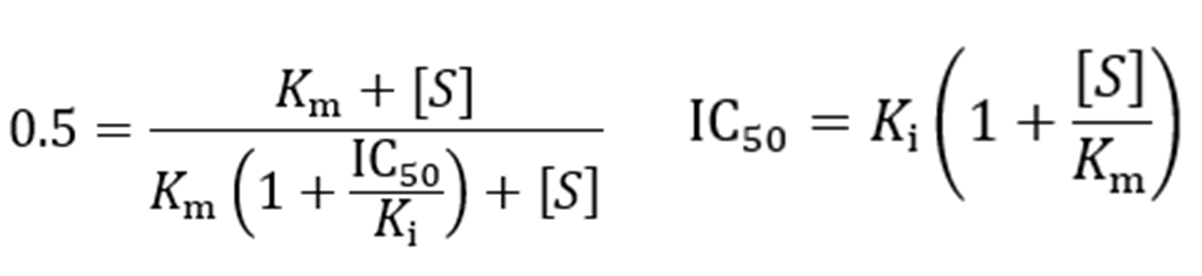
\includegraphics[width=\textwidth]{affinity measurements/IC50.png}
            \end{minipage}   
        \end{figure}
        where
        \begin{itemize}
            \item [S] is the substrate or the molecules that an enzyme acts upon.
            \item [ki] is The kinase Inhibition Constant
            \item [km] is the Michaelis constant is a kinetic parameter, not an equilibrium constant. It gives the substrate concentration at which half of the maximum enzymatic reaction rate is attained. It is determined not only by the substrate’s binding affinity, but also by how quickly the enzyme-substrate complex is turned over into product.   
                       \\ It's a measure of the affinity of an enzyme for its substrate.      
        \end{itemize}

\section{Datasets}
    \subsection{davis benchmark dataset}
        \subsubsection{binding affinity measurement}
            davis dataset uses The kinase dissociation constant \textbf{kd} values after transformation into negative logarithm (base 10) logspace (pKd) using equation $pK_d = -\log_{10} (K_d / 1e9)$.
            with values of \textbf{pkd} ranging ranging from 5.0 to 10.8 where (pKd=5) indicates weak or no interaction which corresponds to $kd = 10000 $ nM or nanoMolar.

            \begin{figure}[H]
                \centering
                \begin{minipage}{0.45\textwidth}
                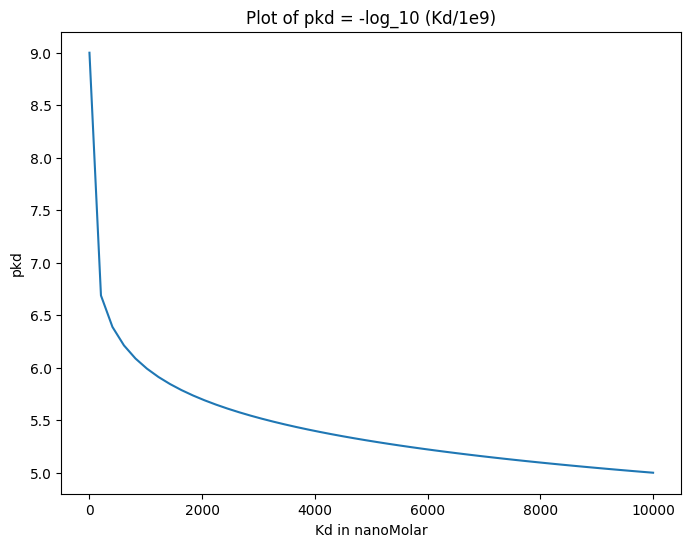
\includegraphics[width=\textwidth]{davis/linear pkd.png}
                \caption{linear}
                \end{minipage}
                \hfill
                \begin{minipage}{0.45\textwidth}
                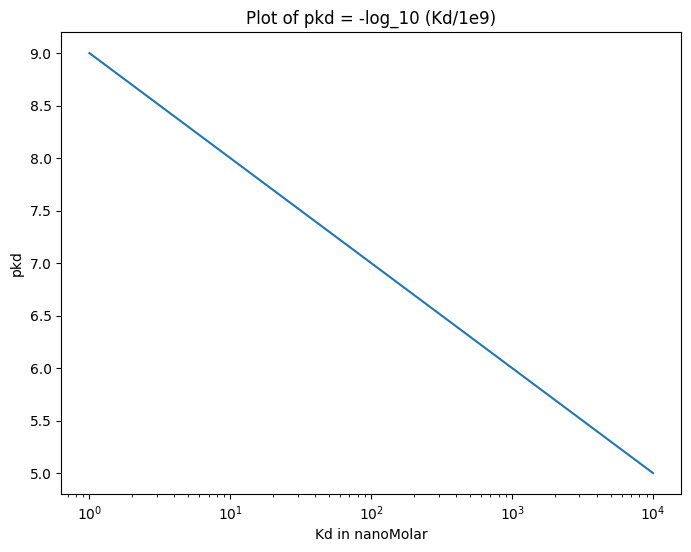
\includegraphics[width=\textwidth]{davis/log pkd.png}
                \caption{log}
                \end{minipage}
            \end{figure}

        \subsubsection{structure}
            contains the pkd binding affinities for all pairs of 68 drugs and 442 targets, total of 30056 interactions
            25047 train set + 5011 test set.
            69\% of which have affinity values of 10000 nM (pKd=5) indicating weak or no interaction.
            \begin{figure}[H]
                \centering
                \begin{minipage}{0.45\textwidth}
                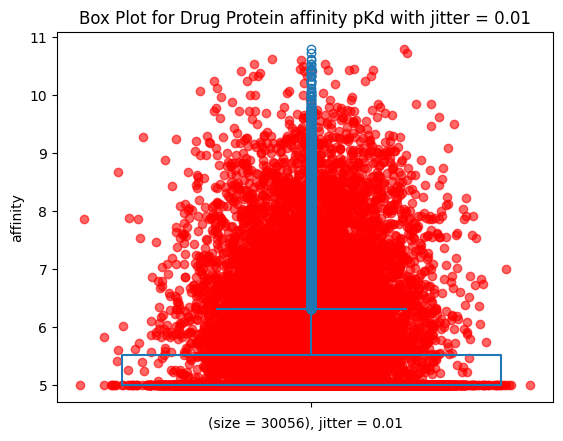
\includegraphics[width=\textwidth]{davis/boxplot.png}
                \end{minipage}
                \hfill
                \begin{minipage}{0.45\textwidth}
                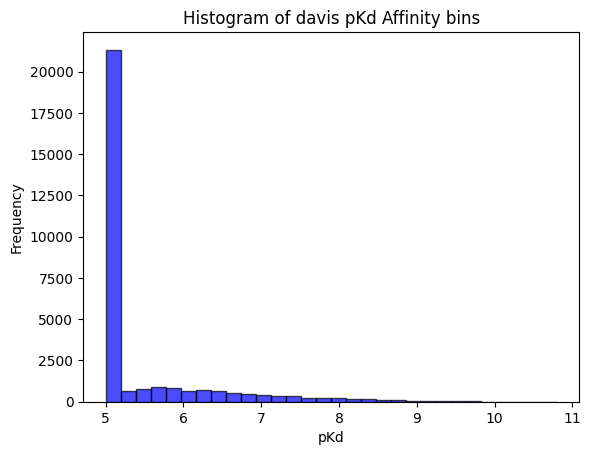
\includegraphics[width=\textwidth]{davis/histogram.png}
                \end{minipage}
            \end{figure}

            also some statistics about davis dataset below show the histogram distribution of SMILES notation and protein sequence with respect to number of characters 

            \begin{figure}[H]
                \centering
                \begin{minipage}{0.45\textwidth}
                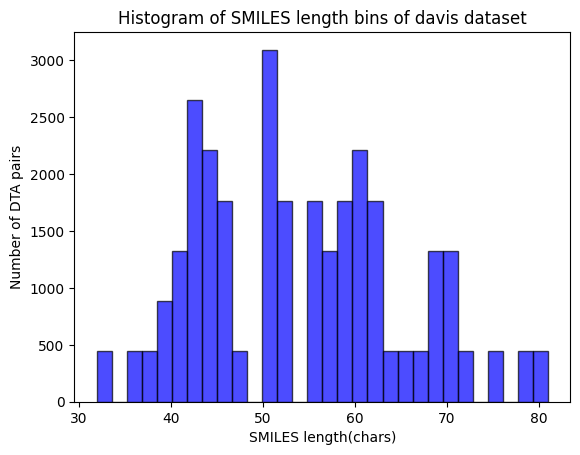
\includegraphics[width=\textwidth]{davis/smiles histogram.png}
                \end{minipage}
                \hfill
                \begin{minipage}{0.45\textwidth}
                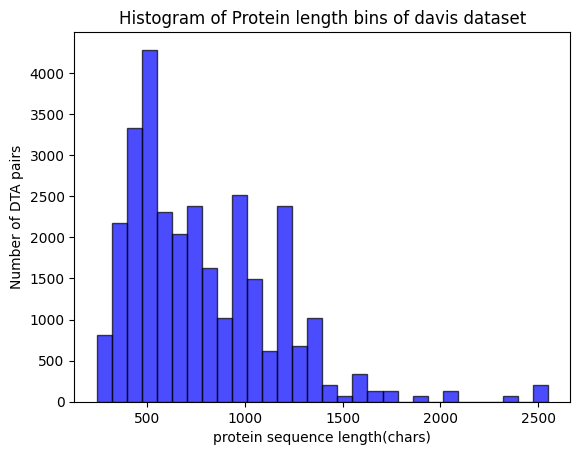
\includegraphics[width=\textwidth]{davis/protein histogram.png}
                \end{minipage}
            \end{figure}

    \subsection{kiba benchmark dataset}
        \subsubsection{binding affinity measurement}
            kiba dataset uses the so called KIBA score which is the integration of heterogeneous information from IC50, Ki , and Kd measurements into a single bioactivity score called by the 
            following adjustments
                \begin{center}
                    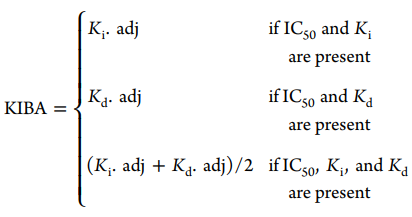
\includegraphics[width=0.4\textwidth]{kiba/kiba adjustments.png}
                \end{center}
        \subsubsection{structure}
            measured as KIBA scores and ranging from 0.0 least affinity to 17.2 highest affinity
            Total of 118257 interactions(98547 train set + 19710 test set)
            most interactions between 10 and 15 kiba score
            \begin{figure}[H]
                \centering
                \begin{minipage}{0.45\textwidth}
                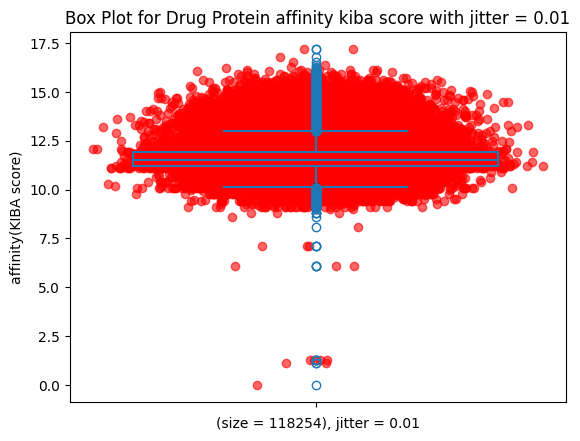
\includegraphics[width=\textwidth]{kiba/boxplot.png}
                \end{minipage}
                \hfill
                \begin{minipage}{0.45\textwidth}
                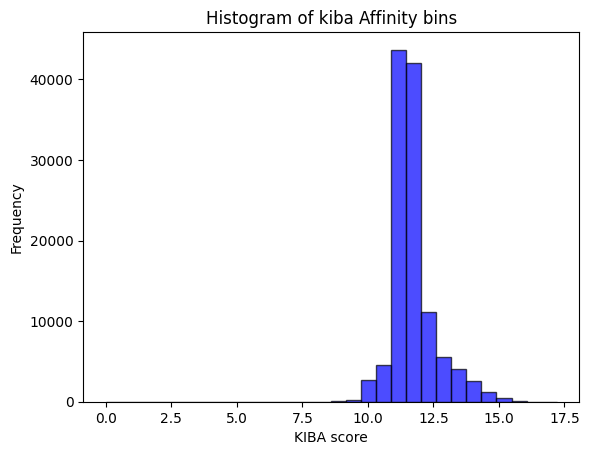
\includegraphics[width=\textwidth]{kiba/histogram.png}
                \end{minipage}
            \end{figure}
            KIBA, on the other hand, has about three-times more interactions with KIBA scores. KIBA values are computed from the
            combination of heterogenous information sources such as IC50, Ki and Kd. the filtered version of the KIBA
            dataset is used, in which each protein and ligand has at least ten interactions. 

            also some statistics about kiba dataset below show the histogram distribution of SMILES notation and protein sequence with respect to number of characters 

            \begin{figure}[H]
                \centering
                \begin{minipage}{0.45\textwidth}
                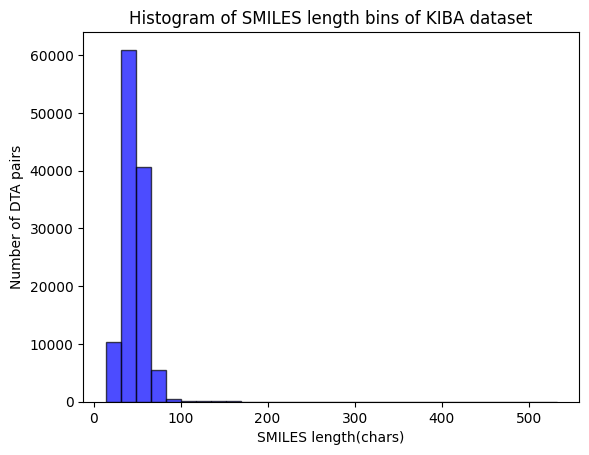
\includegraphics[width=\textwidth]{kiba/smiles histogram.png}
                \end{minipage}
                \hfill
                \begin{minipage}{0.45\textwidth}
                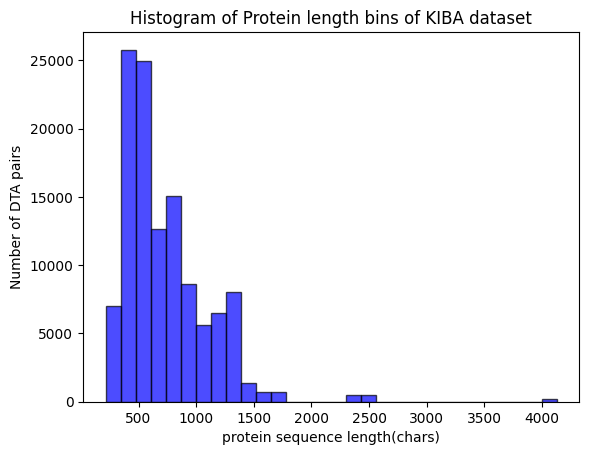
\includegraphics[width=\textwidth]{kiba/protein histogram.png}
                \end{minipage}
            \end{figure}

    \subsection{URV dataset}
        \subsubsection{binding affinity measurement}
        In URV-May-2024 database, the URV systematically collected all structures from the Protein Data Bank (PDB) \cite{11} containing the SARS-CoV-2 Mpro protein - also known as the main protease or 3CL protease, is a key enzyme in the replication and transcription of the SARS-CoV-2 virus, which causes COVID-19 -, devoid of mutations and crystallized with a non-covalent inhibitor. 
        Subsequently, we refined this dataset by selecting structures with available IC50 values from ChEMBL \cite{12} and BindingDB \cite{13} databases, resulting in a final set of 233 structures. 
        For each structure, we obtained the inhibitor's structure in SDF format, the protein-inhibitor complex in PDB format, and the corresponding IC50 value for Mpro inhibition.
        IC50 represents the concentration of inhibitor required to inhibit 50\% of enzyme activity. Additionally, we transformed IC50 values into pIC50, the negative logarithm (base 10) of the IC50 value, where a higher pIC50 value indicates a more potent inhibitor.
        \subsubsection{structure}
        affinity values are provided and some statistics about them are provided below but the measurement unit is unknown.

        affinity values are provided in csv file linked with protein ID and the protein ID in turn is found in the names of the files of both ligand and the protein

        the following figures explain statistics of the affinity values of the 322 pairs, note that jitter was added to one version of the box plot for the sake of clarity
        
        \begin{figure}[H]
            \centering
            \begin{minipage}{0.45\textwidth}
            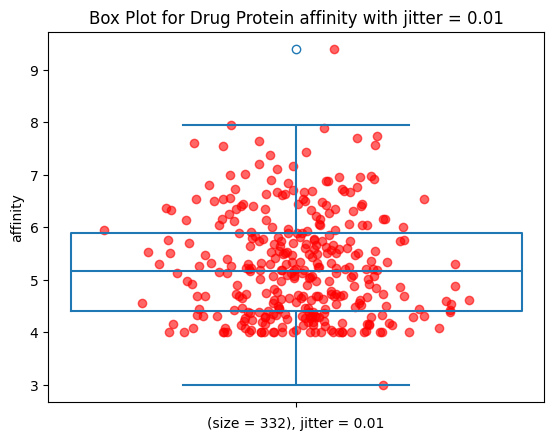
\includegraphics[width=\textwidth]{boxplot2.png}
            \end{minipage}
            \hfill
            \begin{minipage}{0.45\textwidth}
            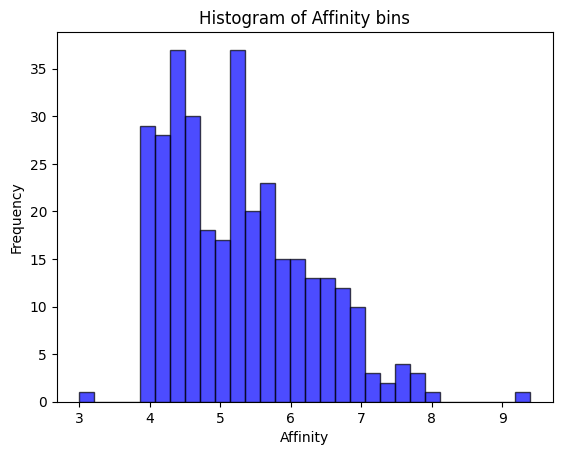
\includegraphics[width=\textwidth]{histogram.png}
            \end{minipage}
        \end{figure}

        also some statistics about URV dataset below show the histogram distribution of SMILES notation and protein sequence with respect to number of characters

        \begin{figure}[H]
            \centering
            \begin{minipage}{0.45\textwidth}
            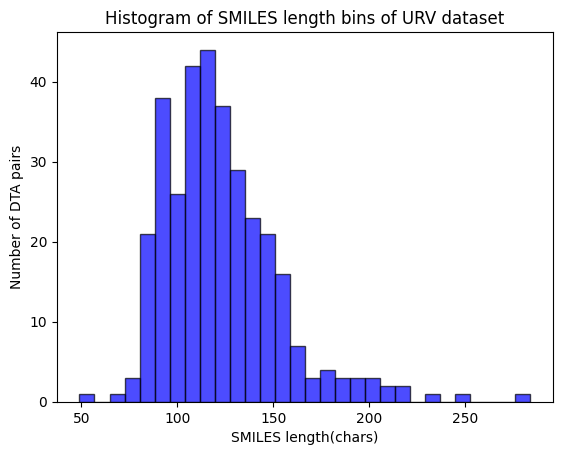
\includegraphics[width=\textwidth]{URV/smiles histogram.png}
            \end{minipage}
            \hfill
            \begin{minipage}{0.45\textwidth}
            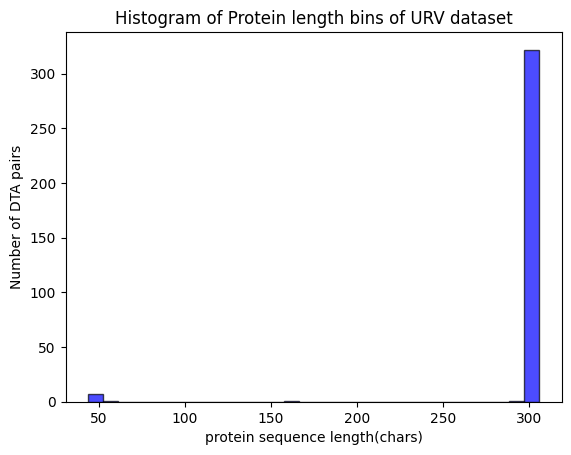
\includegraphics[width=\textwidth]{URV/protein histogram.png}
            \end{minipage}
        \end{figure}

        \subsubsection{protein preprocessing}
        the protein data are initially provided as \textbf{Protein Data Bank(PDB)} files. PDB is a file format used to store 3D structural information about proteins. It is one of the most widely used formats for representing and exchanging structural data in bioinformatics and structural biology.
        PDB files contain atomic coordinates of atoms in a molecule, along with metadata and additional information such as experimental methods used to determine the structure.

        the PDB file name is named after the protein ID. if a PDB file e.g. \textbf{6M2N\_protein.pdb}  is open with any text editor e.g. notepad++, the metadata including its ID, name, type
        are in the header and title tags as shown in figure \ref{fig 2} for protein ID \textbf{6M2N} 

            \begin{figure}[H]
                \centering
                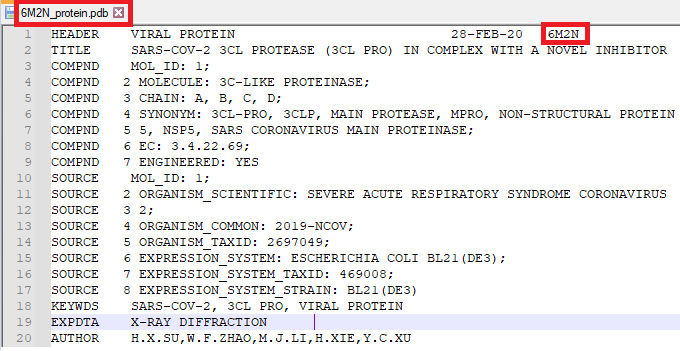
\includegraphics[width=0.75\textwidth]{pdb file.png} % Replace 'example-image' with the path to your image file
                \caption{PDB file example.}
                \label{fig 2}
            \end{figure}

        more informtion can be viewed at the PDB website \cite{4} for the same protein ID \textbf{6M2N}
            \begin{figure}[H]
                \centering
                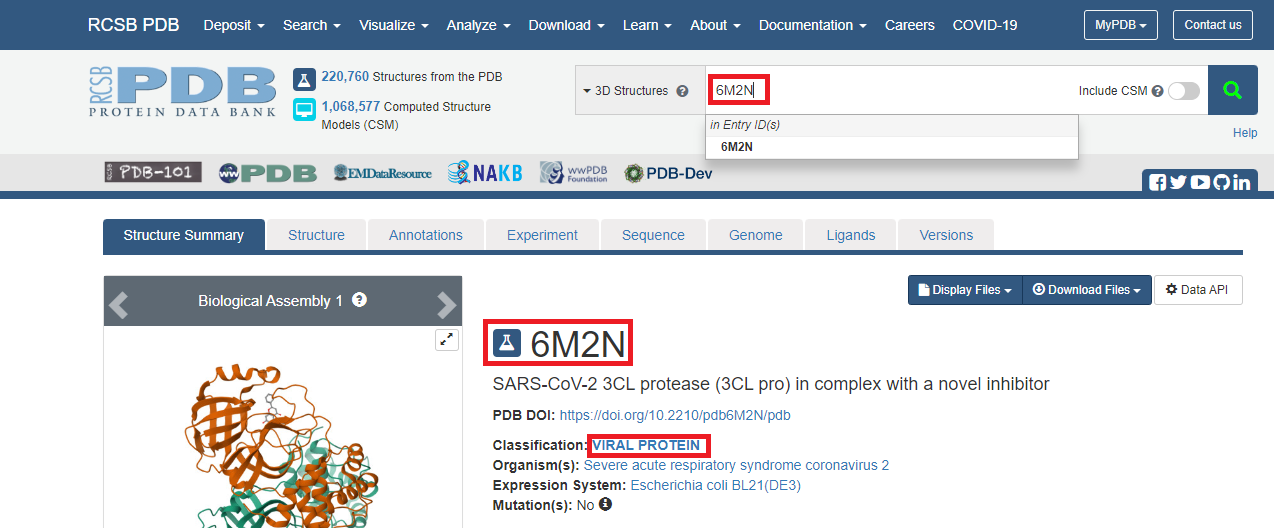
\includegraphics[width=0.75\textwidth]{pdb website.PNG} % Replace 'example-image' with the path to your image file
                \caption{PDB file example.}
                \label{fig 3}
            \end{figure}

        a protein can be either Single Chain or Multi-Chain, so it can be composed of one chain of amino acids(sequence) - up to four - but usually two, we pick the longest sequence as the representation for the protein
        this is done using \textbf{Bio.PDB} module in the \textbf{Biopython} library that provides tools for working with Protein Data Bank (PDB) files in python. classes used are:
        \begin{itemize}
            \item \textbf{PDBParser} used to parse PDB files, create a structure object and read the atomic coordinates and other structural information from a PDB file and converts it into a hierarchical structure object, which can be easily manipulated and analyzed. 
            \item \textbf{PDBBuilder} used to identify and construct polypeptides (chains of amino acids) from a structure object (such as a protein structure obtained from a PDB file)             
        
            \begin{figure}[H]
                \centering
                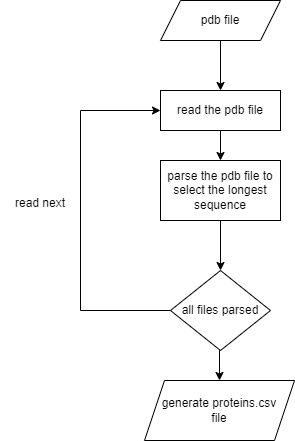
\includegraphics[width=0.4\textwidth]{pdb parser.png} % Replace 'example-image' with the path to your image file
                \caption{PDB file example.}
                \label{fig 4}
            \end{figure}

        \end{itemize} 

        \subsubsection{drug(ligand) preprocessing}
        the ligand data are provided as \textbf{Structure Data file(SDF)} file format used for representing chemical compounds and their associated data. It is primarily used to store information about molecules, including their structure and various properties, in a structured way.

        the SDF file name is named after the protein ID with which the ligand is paired. consider SDF file \textbf{6M2N\_ligand.sdf} shown in fig \ref{fig 5} where its name does not indicate any information about the ligand but suggests it will be paired with previous protein
        to get information about the ligand itself, it can be open using a text editor e.g. notepad++ and at the end of the file information that identify the ligand can be found e.g. \textbf{chemical formula} and \textbf{Simplified Molecular Input Line Entry System(SMILES)} notation which is is a chemical notation that allows a user to represent a chemical structure in a way that can be used by the computer.
        
        \begin{figure}[H]
            \centering
            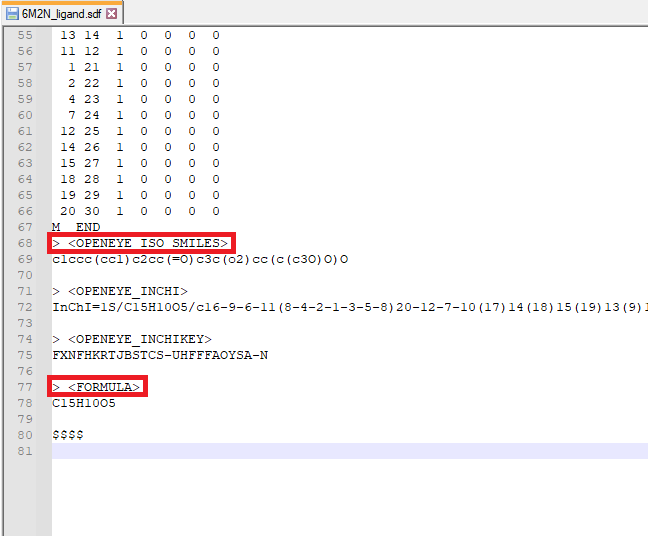
\includegraphics[width=0.7\textwidth]{sdf file.PNG} % Replace 'example-image' with the path to your image file
            \caption{SDF file example.}
            \label{fig 5}
        \end{figure}

        while the chemical formula may not be unique, the SMILES notation is always unique. so it can be used in many websites e.g. the chemspider website\cite{6}  to search for more information about the ligand

        \begin{figure}[H]
            \centering
            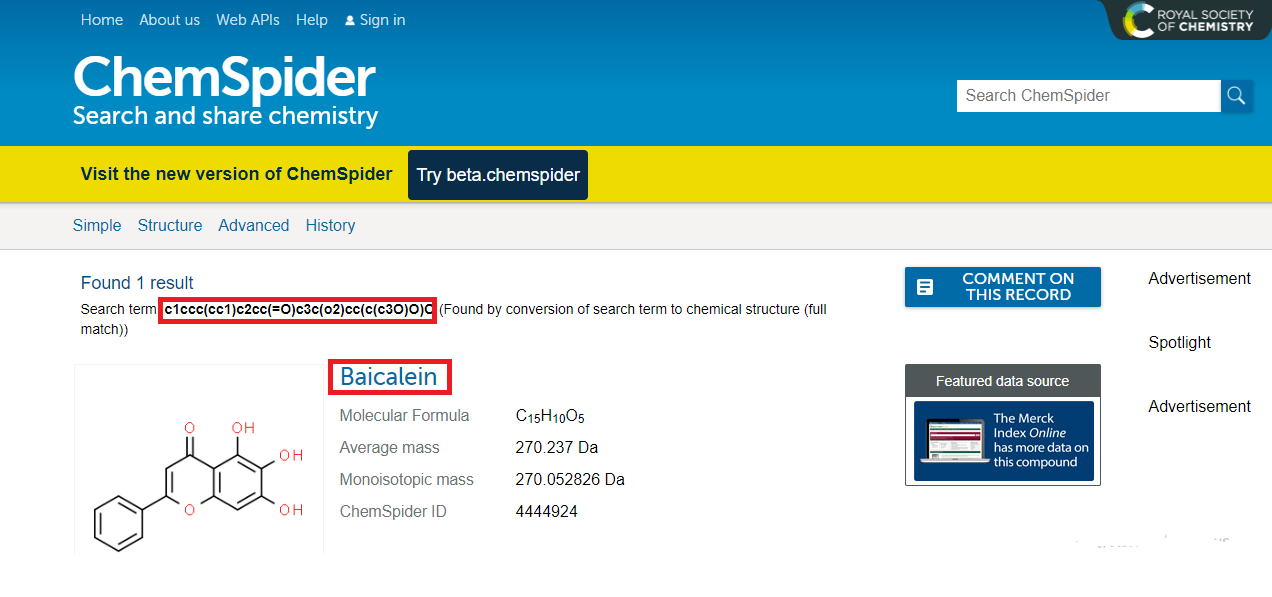
\includegraphics[width=0.9\textwidth]{sdf website.PNG} % Replace 'example-image' with the path to your image file
            \caption{SDF website.}
            \label{fig 6}
        \end{figure}

        An SDF ligand file is read and first the molecule is validated(sanitized) to check if error exist in the structure, if the structure is valid the SMILES notation
        is extracted and appended to valid ligands SDF file else it is excluded and added to invalid ligands SDF file.

        The \textbf{rdkit.Chem} package \cite{7} was used to read the molecule using Chem.SDMolSupplier function, validate it using Chem.SanitizeMol and convert it to SMILES notation
        using function Chem.MolToSmiles

        \begin{itemize}
            \item \textbf{Chem.SDMolSupplier} used to read the molecule.
            \item \textbf{Chem.SanitizeMol} used to validate the molecule             
            \item \textbf{Chem.MolToSmiles} obtain the SMILES notation of the molecule 
        \end{itemize}

        \begin{figure}[H]
            \centering
            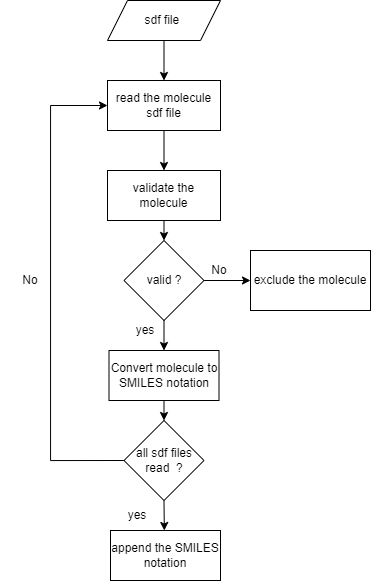
\includegraphics[width=0.5\textwidth]{sdf parser.png} % Replace 'example-image' with the path to your image file
            \caption{SDF workflow.}
            \label{fig 7}
        \end{figure}

        \section{Previous Work and contribution}
        \subsection{Previous Work}
            \subsubsection{collaborative filtering (2017) \cite{8}} 
                The SimBoost model uses the affinity similarities among drugs and among targets to build new features.
                collaborative filtering is used in the following way:
                \begin{itemize}
                    \item Gradient Boosting Machines (GBM): 
                    GBMs are powerful machine learning models that can capture complex relationships between features. SimBoost uses GBMs to learn the relationship between drug similarity, target similarity, and binding affinity.
                    \item Similarity-Based Approach: 
                    SimBoost utilizes a similarity measure to identify drugs and targets that are similar to the query drug and target. This allows the model to leverage existing data on similar compounds and targets to make predictions for new ones.
                    \item Read-Across: 
                    By combining GBMs with a similarity-based approach, SimBoost performs a "read-across" from known data to predict binding affinities for new drug-target pairs.
                \end{itemize}
            \subsubsection{DeepDTA model (2018) \cite{9}}
                DeepDTA uses a deep neural network architecture with two branches to learn complex relationships between drug and target features. It combines:
                \begin{itemize}
                    \item convolutional neural networks (CNNs):
                         for capturing local patterns in molecular structures of drugs.
                    \item recurrent neural networks (RNNs):
                         for capturing sequential information in protein sequences.
                \end{itemize}
                protein representation learned from RNN then combined with the drug representations learned by CNN to predict the binding affinity.
            \subsubsection{WideDTA model (2019) \cite{10}}
                WIDEDTA uses CNNs to learn complex patterns from both the drug SMILES notation and target protein sequence representations. CNNs are particularly well-suited for capturing local patterns in molecular structures and protein sequences.
                in which the sequences of the drugs and proteins are first summarized as higher-order features.\\
                WIDEDTA is considered an extension to and outperforms DEEPDTA. 
    
    
        \subsection{Contribution}
            \subsubsection{GraphDTA paper (2020)}
            a graph neural network architecture capable of directly modeling drugs as molecular graphs outperforms previous deep learning models.
            so This paper tests the hypothesis that a graph structure could yield a better representation for drugs
            directly modeling drugs as molecular graphs and the results show that it outperforms previous deep learning models
 
            \begin{figure}[H]
                \centering
                \begin{minipage}{0.45\textwidth}
                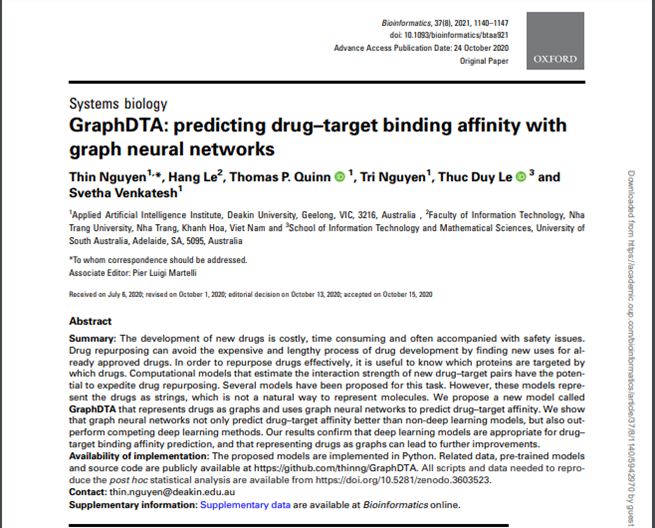
\includegraphics[width=\textwidth]{DTA overview.png}
                \end{minipage}   
            \end{figure}
            
            \subsubsection{Work done in the thesis}
            the work done includes the following:
            \begin{itemize}
                \item \textbf{fork the repository}: 
                \\first the repository of the GraphDTA paper was forked in order to run the code and view the results.
                \begin{figure}[H]
                    \centering
                    \begin{minipage}{0.7\textwidth}
                    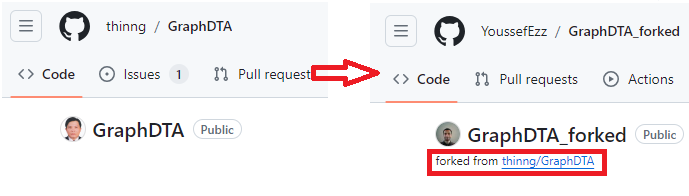
\includegraphics[width=\textwidth]{fork.PNG}
                    \end{minipage}   
                \end{figure}

                \item \textbf{code refactoring}: 
                \\second the code was refactored by writing several functions such as Train, Test and generate the URV database in order to write python notebook files that facilitates tuning the parameters and plotting the results by calling these functions instead of just using commands in terminal.
                \begin{figure}[H]
                    \centering
                    \begin{minipage}{0.8\textwidth}
                    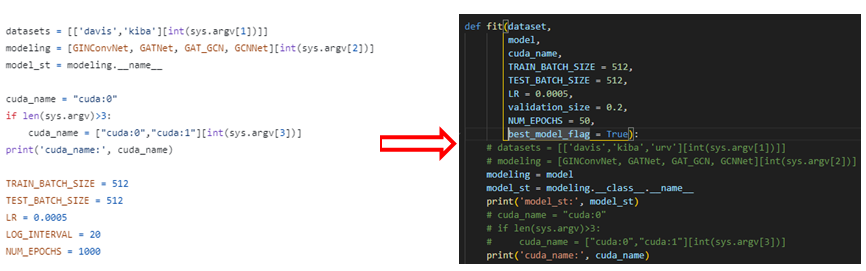
\includegraphics[width=\textwidth]{refactor.png}
                    \end{minipage}   
                \end{figure}

                \end{itemize}

\section{GraphDTA Network architecture}
    The overall architecture combines the information from the molecular graph and the protein sequence to make a prediction. it is a PyTorch implementation of a Graph Convolutional Network (GCN) based model

    \begin{center}
        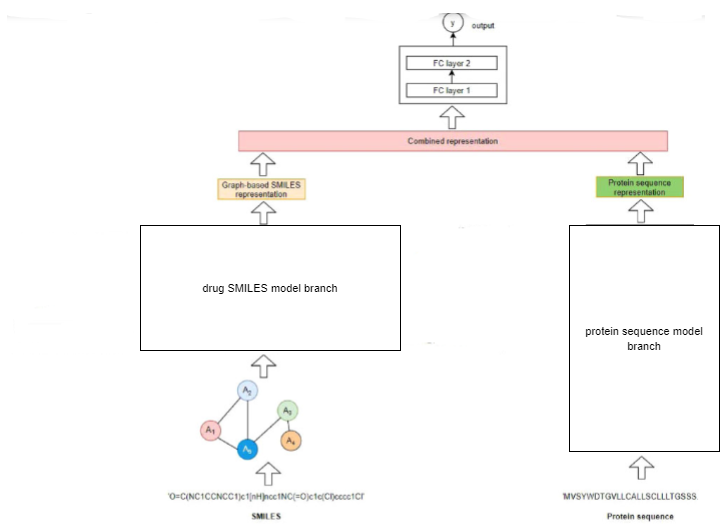
\includegraphics[width=0.8\textwidth]{model/architecture.drawio.png}
    \end{center}

    The architecture consists of two main branches the protein branch and the drug branch

    \subsection{Protein sequence branch}
    operates on the protein sequence input, which is represented as a sequence of integer indices of characters representing amino acids and the steps of processing are as follows:
        \begin{center}
            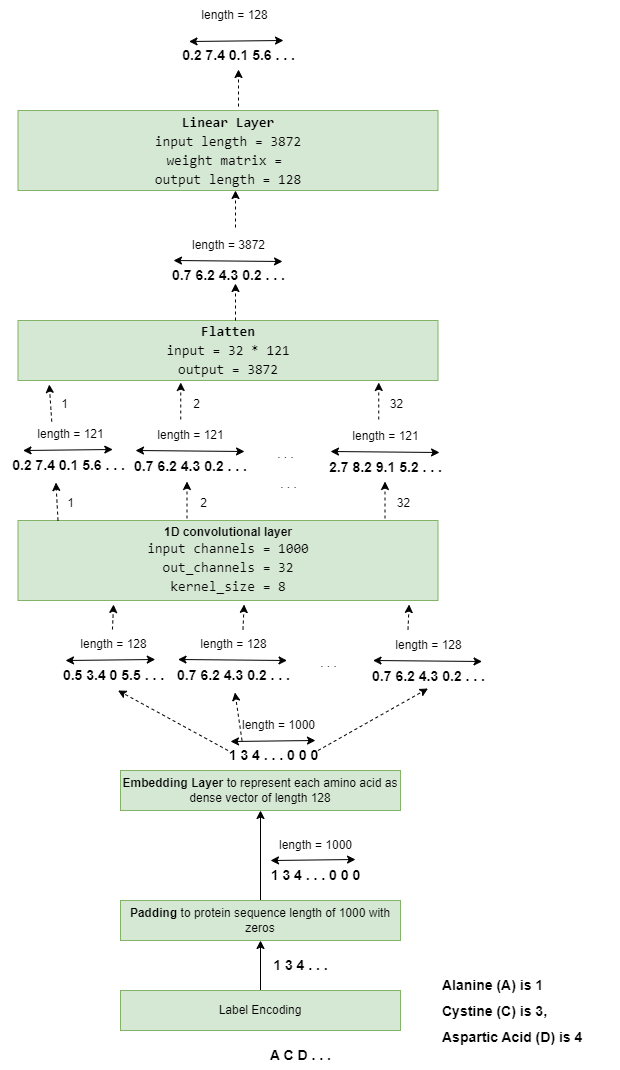
\includegraphics[width=0.7\textwidth]{model/Protein branch.drawio.png}
        \end{center}
        \begin{enumerate}
            \item \textbf{initial representation}: The protein sequence is a string of ASCII characters which represent amino acids.
            \item \textbf{label encoding}: Each amino acid type is encoded with an integer based on its associated alphabetical symbol [e.g. Alanine (A) is 1, Cystine (C) is 3, Aspartic Acid (D) is 4 and so on], allowing the protein to be represented as an integer sequence. 
            \item \textbf{padding}: the sequence is cut or padded to a fixed length sequence of 1000 residues. In case a sequence is shorter, it is padded with zero values.
            \item \textbf{embedding layer}: The protein sequence is passed through an embedding layer (embedding\_xt) to convert the integer indices into a dense vector representation.
            \item \textbf{1D convolutional layer}: The embedded sequence is then passed through a 1D convolutional layer (conv\_xt\_1) to extract features from the protein sequence.
            \item \textbf{flattening}: The convolutional features are flattened and passed through a fully connected layer (fc1\_xt) to obtain a fixed size output representation.
            \item \textbf{linear layer}: The line effectively creates a linear layer that will take an input of size 3872 (the flattened output from the convolution) and produce an output of size 128
        \end{enumerate} 

    \subsection{SMILES graph branch}
        operates on the molecular graph representation of the input SMILES. could be any of four models
        
            \subsubsection{GCN-based model}
                
                it uses graph convolutional(GCN) operater from paper ``Semi-supervised Classification with Graph Convolutional Networks.'' in 2017 and it is impemented in torch geometric as \textbf{GCNConv}
                \begin{figure}[H]
                    \centering
                    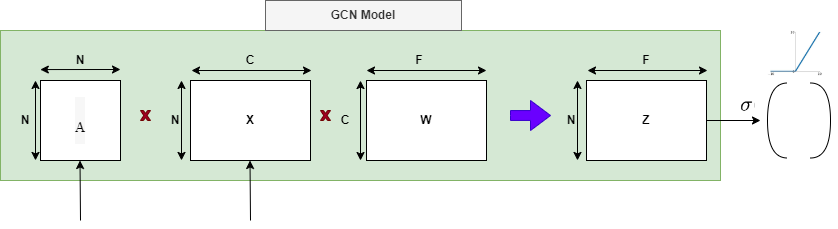
\includegraphics[width=0.9\textwidth]{model/GCN_Model.drawio.png} % Replace 'example-image' with the path to your image file
                    \caption{GCN operator}
                \end{figure}

                \begin{itemize}
                    \item \textbf{A} is the normalized adjacency matrix \textbf{N * N}
                    \item \textbf{X} is node feature matrix \textbf{N * C}
                    \item \textbf{W} weight matrix of size \textbf{C * F}
                    \item \textbf{Z} node-level output matrix \textbf{N * F}
                \end{itemize}

                \begin{figure}[H]
                    \centering
                    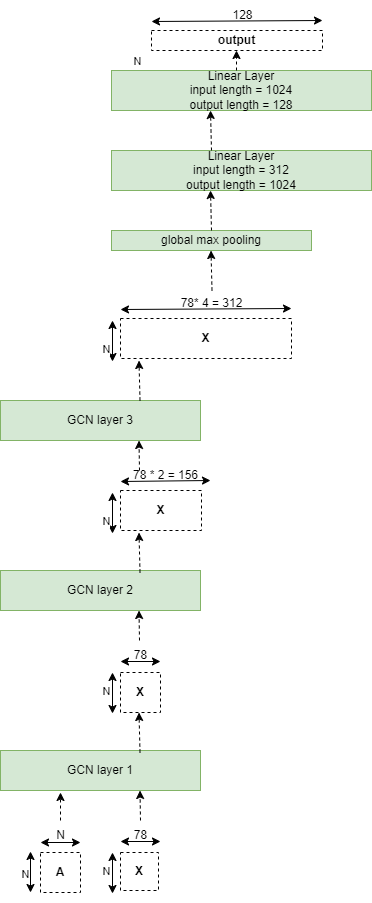
\includegraphics[width=0.5\textwidth]{model/GCN-based.drawio.png} % Replace 'example-image' with the path to your image file
                    \caption{GCN-based model}
                \end{figure}

            \subsubsection{GAT-based model}
                \begin{enumerate}
                    \item The model starts with two GAT layers, gcn1 and gcn2, which operate on the input graph data.
                    \item The first GAT layer, gcn1, takes the initial node features (num\_features\_xd) and outputs a representation with 10 heads, effectively increasing the feature dimensionality by a factor of 10.
                    \item The second GAT layer, gcn2, then reduces the feature dimensionality to output\_dim.
                    \item After the GAT layers, a fully connected layer fc\_g1 is applied to the output of the second GAT layer.
                \end{enumerate}

                \begin{center}
                    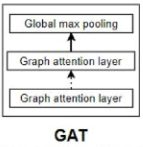
\includegraphics[width=0.3\textwidth]{GAT_model.PNG}
                \end{center}
            
            \subsubsection{GATGCN-based model}
                \begin{enumerate}
                    \item The first layer is a GATConv layer, which implements the Graph Attention Network mechanism. It takes the input node features (num\_features\_xd) and outputs features with the same dimensionality, but with 10 attention heads.
                    \item The second layer is a GCNConv layer, which applies a standard Graph Convolutional Network operation. It takes the concatenated output of the previous GAT layer (10 times the original number of features) and outputs the same number of features.
                \end{enumerate}

                \begin{center}
                    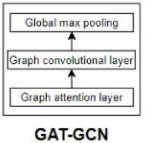
\includegraphics[width=0.3\textwidth]{GAT_GCN.PNG}
                \end{center}
            
            \subsubsection{GIN-based model}
                \begin{enumerate}
                    \item The model has 5 GINConv layers, each with a sequential neural network (nn1, nn2, ..., nn5) that consists of a Linear layer, a ReLU activation, and another Linear layer.
                    \item Each GINConv layer is followed by a BatchNorm1d layer to normalize the output.
                \end{enumerate}

                \begin{center}
                    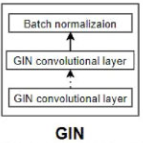
\includegraphics[width=0.3\textwidth]{GIN_model.PNG}
                \end{center}

               
    \subsection{combined fully connected layers}      
        After obtaining the output representations from the two branches -protein and drug -, the model concatenates them and passes the combined features through a regular neural network composed of two fully connected layers linear layers to produce the final output.
        The model uses ReLU activations, dropout for regularization after each linear layer.
        \begin{center}
            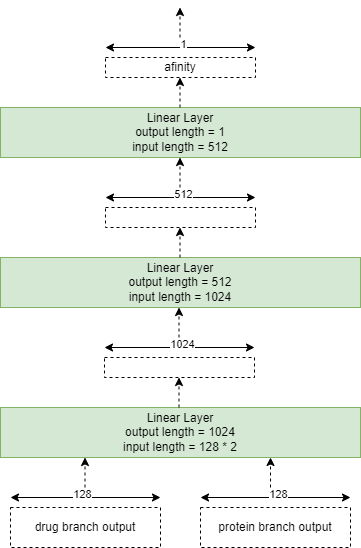
\includegraphics[width=0.5\textwidth]{model/Combined_representation.drawio.png}
        \end{center}

        \begin{enumerate}
            \item \textbf{drug branch output}: tensor of length 128 of the output of the drug graph branch
            \item \textbf{protein branch output}: tensor of length 128 of the output of the protein branch
            \item \textbf{Linear layer 1}: takes as input the concatenation of two tensors of length 256 - 128 each that represent the output of drug and protein branch - and produces a tensor of length 1024 by applying weight matrix 1024 * 256 followed by RELU activation function
            \item \textbf{Linear layer 2}: take as input a tensor of length 1024 which is the output of the first linear layer and produces a tensor of length 512 by applying weight matrix 512 * 1024 followed by RELU activation function
            \item \textbf{Linear layer 3}: take as input a tensor of length 512 which is the output of the second linear layer and produces a tensor of length 1 which is the output affinity by applying weight matrix 1 * 512 
        \end{enumerate} 

\section{Results}
    \subsection{for davis dataset}
        \subsubsection{train and test of GCN-based model}
        by training the network with the parameters suggested by the paper shown we obtain the error loss curve for training and validation set 
        \begin{center}
            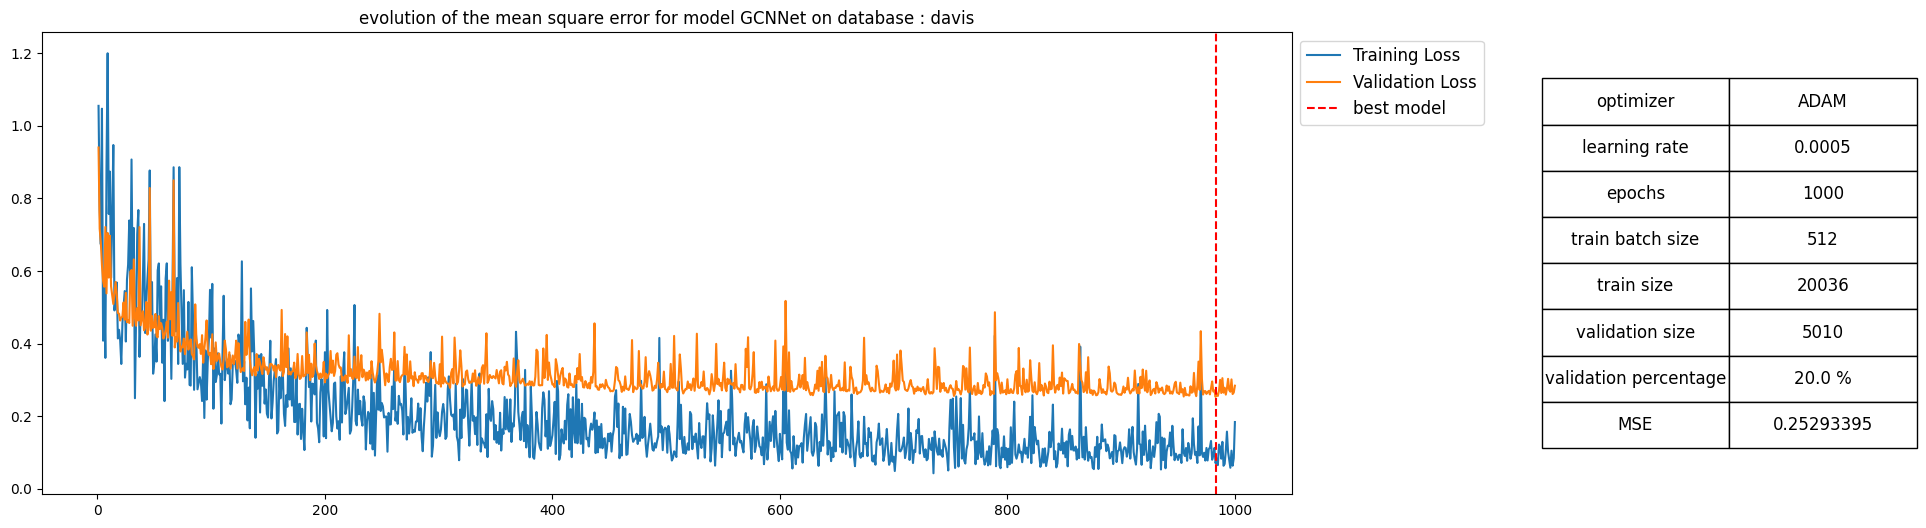
\includegraphics[width=1.0\textwidth]{train_test_plots/davis GCN train.png}
        \end{center}
        and the resulting predicted-actual curve is as follows:
        \begin{center}
            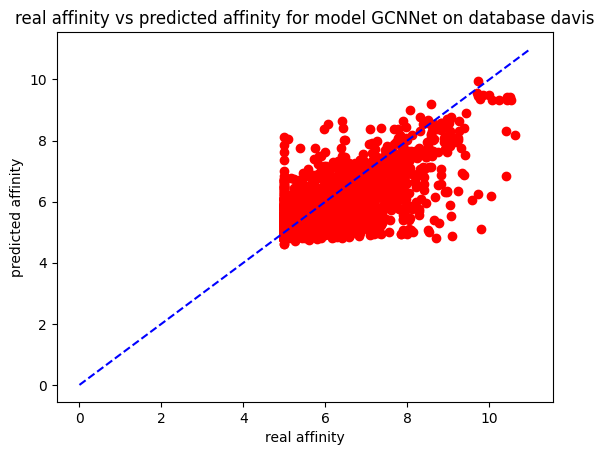
\includegraphics[width=0.6\textwidth]{train_test_plots/davis GCN test.png}
        \end{center}

        \subsubsection{train and test of GATGCN-based model}
        by training the network with the parameters suggested by the paper shown we obtain the error loss curve for training and validation set 
        \begin{center}
            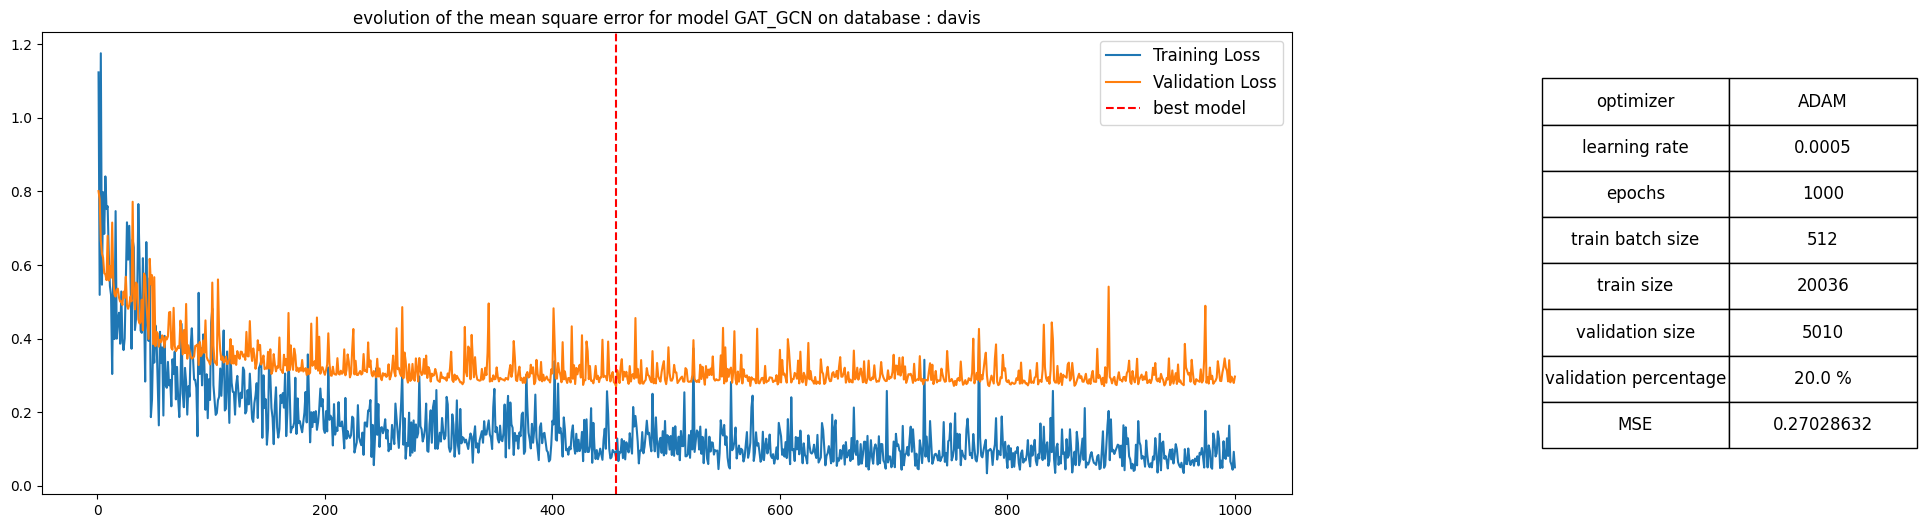
\includegraphics[width=1.0\textwidth]{train_test_plots/davis GATGCN train.png}
        \end{center}
        and the resulting predicted-actual curve is as follows:
        \begin{center}
            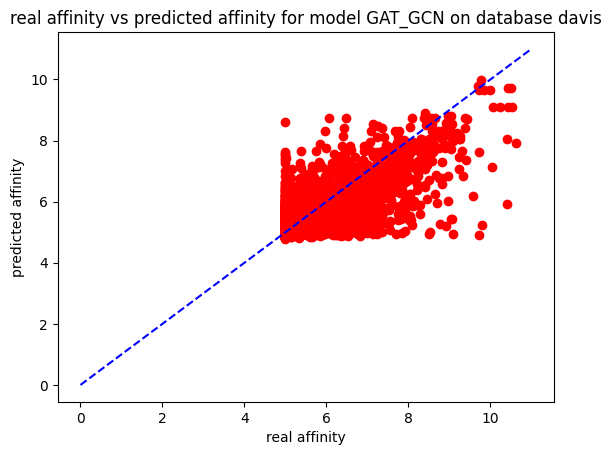
\includegraphics[width=0.6\textwidth]{train_test_plots/davis GATGCN test.png}
        \end{center}

        \subsubsection{train and test GAT-based model}
        by training the network with the parameters suggested by the paper shown we obtain the error loss curve for training and validation set 
        \begin{center}
            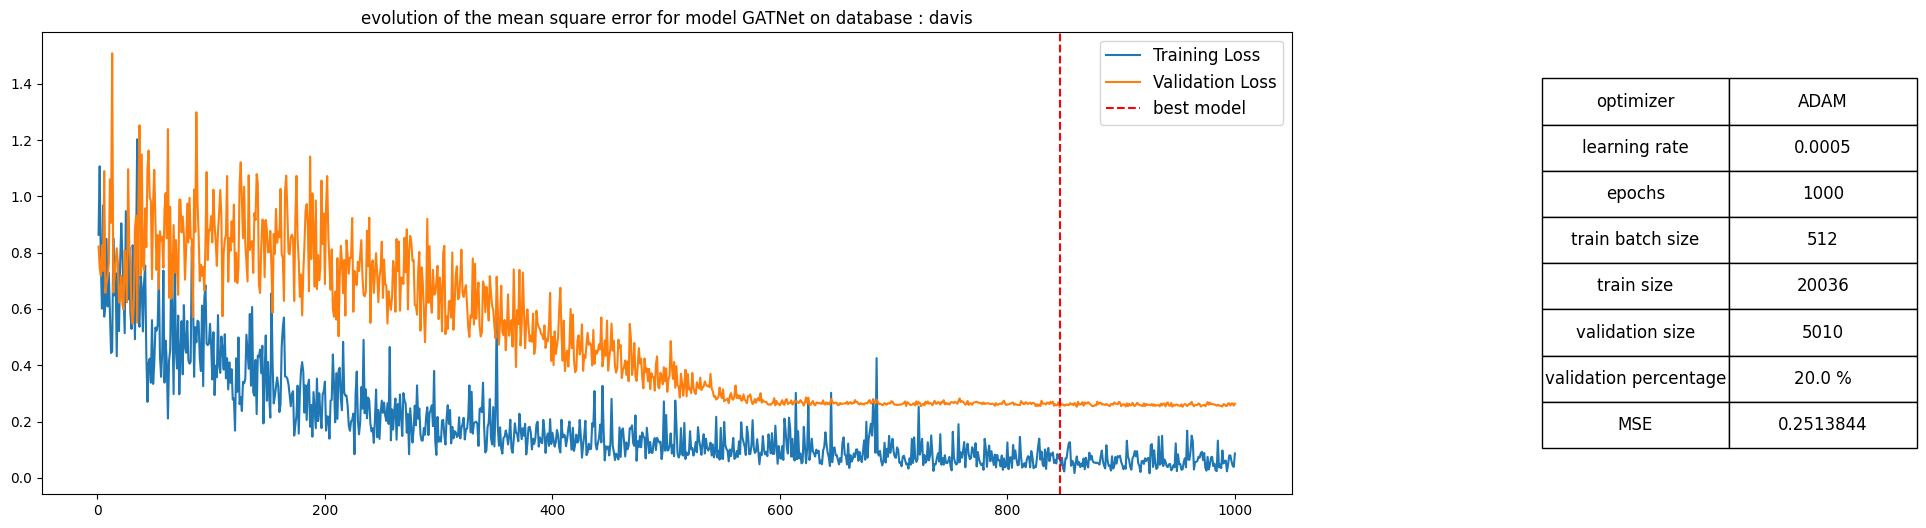
\includegraphics[width=1.0\textwidth]{train_test_plots/davis GAT train.png}
        \end{center}
        and the resulting predicted-actual curve is as follows:
        \begin{center}
            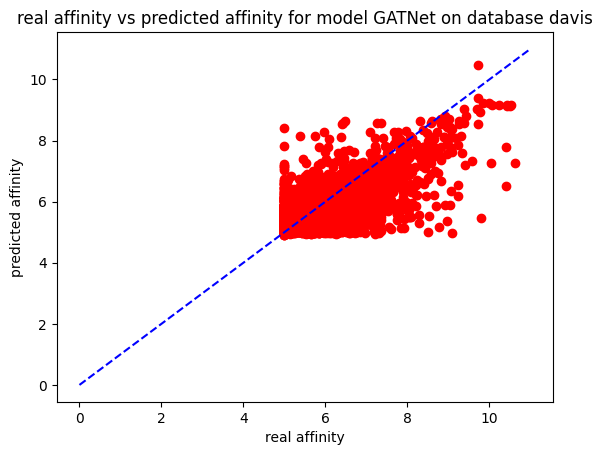
\includegraphics[width=0.6\textwidth]{train_test_plots/davis GAT test.png}
        \end{center}

        \subsubsection{train and test GINCONV-based model}
        by training the network with the parameters suggested by the paper shown we obtain the error loss curve for training and validation set 
        \begin{center}
            \includegraphics[width=1.0\textwidth]{train_test_plots/davis GInCONV train.png}
        \end{center}
        and the resulting predicted-actual curve is as follows:
        \begin{center}
            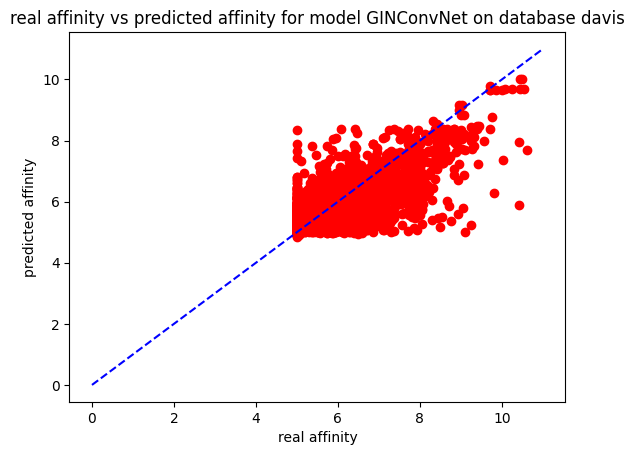
\includegraphics[width=0.6\textwidth]{train_test_plots/davis GINCONV test.png}
        \end{center}
    
    \subsection{for kiba dataset}
        \subsubsection{train and test GCN-based model}
        by training the network with the parameters suggested by the paper shown we obtain the error loss curve for training and validation set 
        \begin{center}
            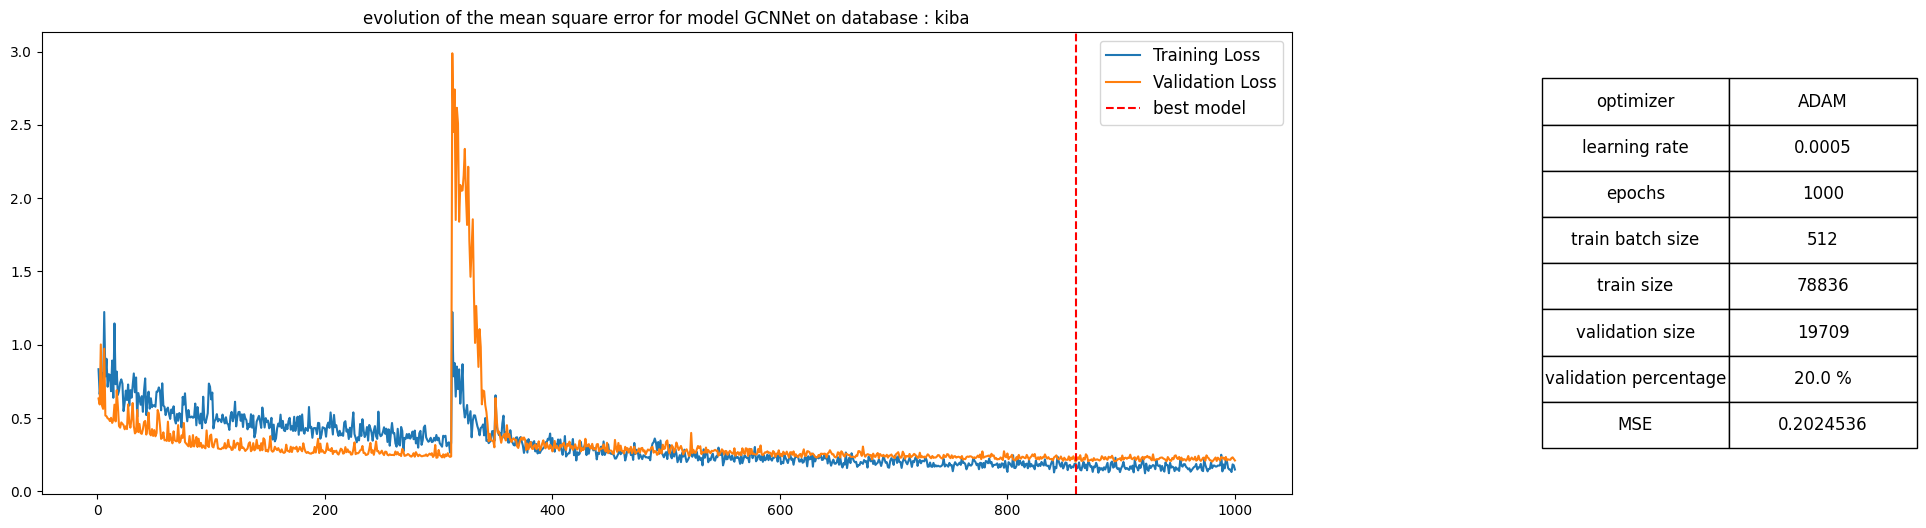
\includegraphics[width=1.0\textwidth]{train_test_plots/kiba GCN train.png}
        \end{center}
        and the resulting predicted-actual curve is as follows:
        \begin{center}
            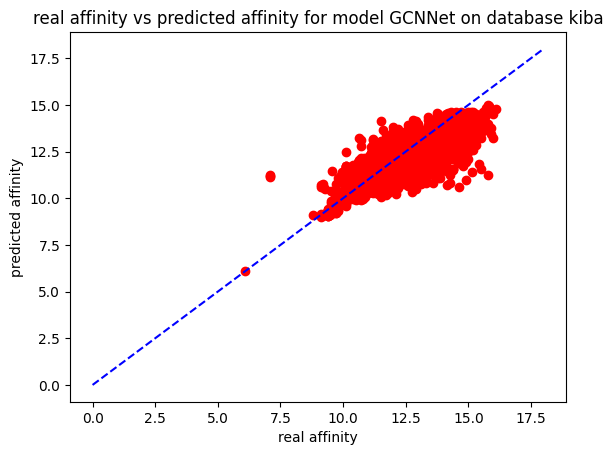
\includegraphics[width=0.6\textwidth]{train_test_plots/kiba GCN test.png}
        \end{center}

        \subsubsection{train and test GATGCN-based model}
        by training the network with the parameters suggested by the paper shown we obtain the error loss curve for training and validation set 
        \begin{center}
            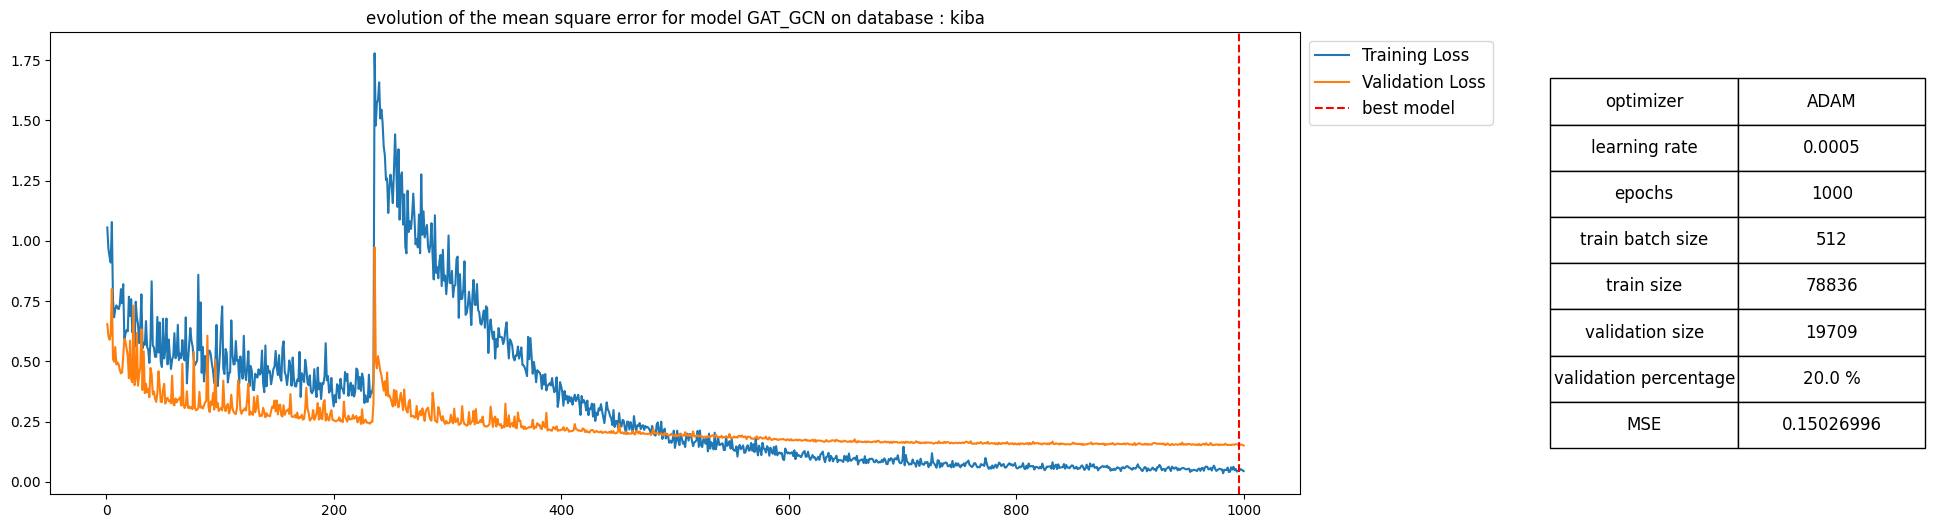
\includegraphics[width=1.0\textwidth]{train_test_plots/kiba GATGCN train.png}
        \end{center}
        and the resulting predicted-actual curve is as follows:
        \begin{center}
            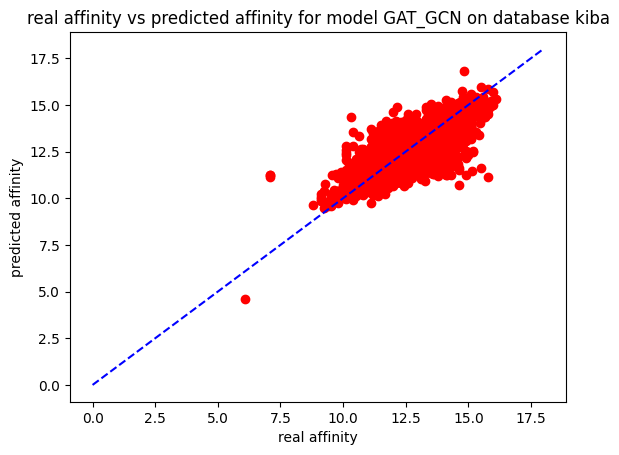
\includegraphics[width=0.6\textwidth]{train_test_plots/kiba GATGCN test.png}
        \end{center}

        \subsubsection{train and test GAT-based model}
        by training the network with the parameters suggested by the paper shown we obtain the error loss curve for training and validation set 
        \begin{center}
            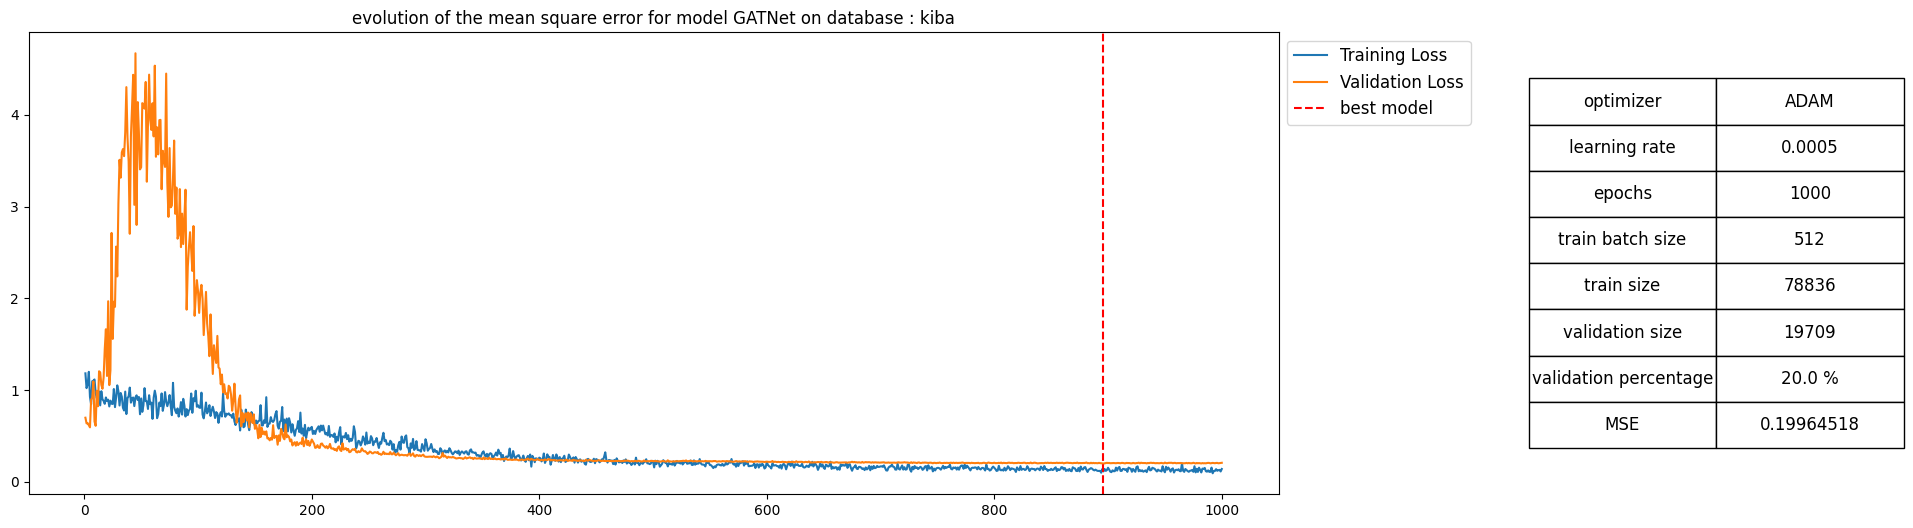
\includegraphics[width=1.0\textwidth]{train_test_plots/kiba GAT train.png}
        \end{center}
        and the resulting predicted-actual curve is as follows:
        \begin{center}
            \includegraphics[width=0.6\textwidth]{train_test_plots/kiba GAT test.png}
        \end{center}

        \subsubsection{train and test GINCONV-based model}
        by training the network with the parameters suggested by the paper shown we obtain the error loss curve for training and validation set 
        \begin{center}
            \includegraphics[width=1.0\textwidth]{train_test_plots/kiba GINCONV train.png}
        \end{center}
        and the resulting predicted-actual curve is as follows:
        \begin{center}
            \includegraphics[width=0.6\textwidth]{train_test_plots/kiba GINCONV test.png}
        \end{center}
    
    \subsection{for URV dataset}
        \subsubsection{train and test GCN-based model}
        by training the network while tuning the parameters starting with those suggested by the paper shown we obtain the error loss curve for training and validation set 
        \begin{center}
            \includegraphics[width=1.0\textwidth]{train_test_plots/URV GCN train.png}
        \end{center}
        and the resulting predicted-actual curve is as follows:
        \begin{center}
            \includegraphics[width=0.6\textwidth]{train_test_plots/URV GCN test.png}
        \end{center}

        \subsubsection{train and test GATGCN-based model}
        by training the network while tuning the parameters starting with those suggested by the paper shown we obtain the error loss curve for training and validation set 
        \begin{center}
            \includegraphics[width=1.0\textwidth]{train_test_plots/URV GATGCN train.png}
        \end{center}
        and the resulting predicted-actual curve is as follows:
        \begin{center}
            \includegraphics[width=0.6\textwidth]{train_test_plots/URV GATGCN test.png}
        \end{center}

        \subsubsection{train and test GAT-based model}
        by training the network while tuning the parameters starting with those suggested by the paper shown we obtain the error loss curve for training and validation set 
        \begin{center}
            \includegraphics[width=1.0\textwidth]{train_test_plots/URV GAT train.png}
        \end{center}
        and the resulting predicted-actual curve is as follows:
        \begin{center}
            \includegraphics[width=0.6\textwidth]{train_test_plots/URV GAT test.png}
        \end{center}

        \subsubsection{train and test GINCONV-based model}
        by training the network while tuning the parameters starting with those suggested by the paper shown we obtain the error loss curve for training and validation set 
        \begin{center}
            \includegraphics[width=1.0\textwidth]{train_test_plots/URV GINCONV train.png}
        \end{center}
        and the resulting predicted-actual curve is as follows:
        \begin{center}
            \includegraphics[width=0.6\textwidth]{train_test_plots/URV GINCONV test.png}
        \end{center}
    
    \subsection{Summary and conclusion}
        the results are summarized in the following table
        \begin{center}
            \includegraphics[width=1.0\textwidth]{summary.png}
        \end{center}
        it was noticed that best MSE was obtained in results of kiba dataset then davis and finally the results of URV dataset - either in paper or in thesis - and this might be due to the following reasons:
        \begin{enumerate}
            \item the sample size of the data including train and test sets is largest in kiba then davis followed by URV and this helps the network learn more robust and generalizable patterns, thus make accurate predictions on unseen data..
            \item kiba dataset has the best diversity specially for the target proteins as it integrates different bioactivity scores and this is crucial to train a model capable of generalizing to unseen drug-target pairs.  
        \end{enumerate}

%\addcontentsline{toc}{section}{Bibliography} % Add Bibliography to TOC
%\printbibliography 
\begin{thebibliography}{3}

\bibitem{1}
    [Thin et al.] Thin Nguyen;  Hang Le; Thomas P. Quinn; Tri Nguyen; Thuc Duy Le; and
    Svetha Venkatesh, "GraphDTA: predicting drug–target binding affinity with
    graph neural networks",
    \\Journal Bioinformatics, Volume 37, Issue 8, March 2021, Pages 1140–1147
    \\Available at
    \url{https://academic.oup.com/bioinformatics/article/37/8/1140/5942970}.

\bibitem{2}
    Related data, pre-trained models and source code in \cite{1} are publicly available at \url{https://github.com/thinng/GraphDTA}.

\bibitem{3}
    the repository forked from \cite{2} to perform experiments in this thesis available at \url{https://github.com/YoussefEzz/GraphDTA_forked}.
\bibitem{4}
PDB website: \url{https://www.rcsb.org/}.

\bibitem{5}
Bio.PDB Biopython module: \url{https://biopython.org/wiki/The_Biopython_Structural_Bioinformatics_FAQ}.

\bibitem{6}
chemspider website: \url{https://www.chemspider.com/}.

\bibitem{7}
rdkit library: \url{https://www.rdkit.org/docs/source/rdkit.Chem.html}.

\bibitem{8}
[He et al.] Tong He; Marten Heidemeyer; Fuqiang Ban; Artem Cherkasov and Martin Ester "SimBoost: a read-across approach
for predicting drug–target binding affinities using gradient boosting machines",
    \\Journal of Cheminformatics, 9, Article number: 24 (2017)
    \\Available at
    \url{https://jcheminf.biomedcentral.com/articles/10.1186/s13321-017-0209-z}.

\bibitem{9}
[Ozturk et al.] Hakime Ozturk; Arzucan Ozgur and Elif Ozkirimli "DeepDTA: deep drug–target binding
affinity prediction",
    \\Journal of Bioinformatics, Volume 34, Issue 17, September 2018, Pages i821–i829,
    \\Available at
    \url{https://academic.oup.com/bioinformatics/article/34/17/i821/5093245}.

\bibitem{10}
[Ozturk et al.] Hakime Ozturk; Arzucan Ozgur and Elif Ozkirimli "WIDEDTA: PREDICTION OF DRUG-TARGET BINDING AFFINITY",
    \\Available at
    \url{https://arxiv.org/abs/1902.04166}.

\bibitem{11}
Berman, H.M., Westbrook, J., Feng, Z., Gilliland, G., Bhat, T.N., Weissig, H., Shindyalov, I.N., Bourne, P.E. (2000). The Protein Data Bank. Nucleic Acids Research, 28(1), 235-242. 
[doi:10.1093/nar/28.1.235]

\bibitem{12}
Zdrazil, B., Felix, E., Hunter, F., et al. (2024). The ChEMBL Database in 2023: a drug discovery platform spanning multiple bioactivity data types and time periods. Nucleic Acids Research, 52(D1), D1180–D1192. 
[doi:10.1093/nar/gkad1004]

\bibitem{13}
Gilson, M. K., Liu, T., Baitaluk, M., et al. (2016). BindingDB in 2015: A public database for medicinal chemistry, computational chemistry and systems pharmacology. Nucleic Acids Research, 44(D1), D1045–D1053. 
[doi:10.1093/nar/gkv1072]

\end{thebibliography}

\end{document}
